\documentclass[tikz]{standalone}

\usepackage{newtxtext,newtxmath}

%!TEX root = main.tex

% mytikzset
\usepackage{tikz}
\usetikzlibrary{positioning,arrows,shapes,patterns}
\usetikzlibrary{decorations.pathmorphing}
\usetikzlibrary{decorations.markings}
\usetikzlibrary{decorations.pathreplacing}
\usetikzlibrary{calc}
\usetikzlibrary{patterns}
\usetikzlibrary{decorations.markings}
\usetikzlibrary{petri}

\tikzset{
  vector/.style={thick,double,draw=black, postaction={decorate},
    decoration={markings,mark=at position .6 with {\arrow[black,scale=0.4]{triangle 45}}}},
  axial/.style={thick,double,densely dashed,draw=black, postaction={decorate},
    decoration={markings,mark=at position .6 with {\arrow[black,scale=0.4]{triangle 45}}}},
  gluon/.style={decorate, draw=black,
    decoration={coil,aspect=0.3,segment length=5pt,amplitude=3pt}},
  pseudo/.style={thick, dashed, draw=black, postaction={decorate},
    decoration={markings,mark=at position .6 with {\arrow[red,scale=0.5]{triangle 45}}}},
  scalar/.style={thick,draw=black, postaction={decorate},
    decoration={markings,mark=at position .6 with {\arrow[black,scale=0.5]{triangle 45}}}},
  cut/.style={draw=black, decorate, decoration={snake, segment length=1mm, amplitude=0.2mm}}
}

\usetikzlibrary{decorations.pathreplacing}

\begin{document}
\nopagecolor
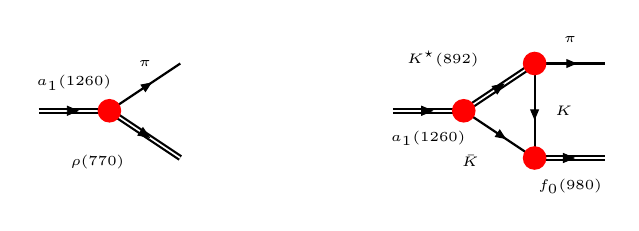
\begin{tikzpicture}[node distance=0.6cm and 0.9cm]
    \coordinate[] (pl2);
    \coordinate[right=of pl2] (a1s);
    \coordinate[right=of a1s] (a2s); 
    \coordinate[above right=of a2s] (b1s); 
    \coordinate[below right=of a2s] (b2s); 
    
    \coordinate[above right=of b2s] (x0); 
    \coordinate[right=of x0] (x1); 

    \coordinate[right=of x1] (a1); 
    \coordinate[right=of a1] (a2); 
    \coordinate[above right=of a2] (b1); 
    \coordinate[below right=of a2] (b2); 
    \coordinate[right      =of b1] (c1);
    \coordinate[right      =of b2] (c2);

     
    \draw[vector] (a1) -- node[label=below:{\tiny $a_1(1260)$} ] {} (a2); 
    \draw[vector] (a2) -- node[label=above left:{\tiny $K^\star(892)$} ] {}(b1); 
    \draw[scalar] (a2) -- node[label=below left:{\tiny $\bar{K}$} ] {} (b2); 
    \draw[scalar] (b1) -- node[label=right:{\tiny $K$} ] {} (b2); 
    \draw[scalar] (b1) -- node[label=above:{\tiny $\pi$} ] {} (c1); 
    \draw[vector] (b2) -- node[label=below:{\tiny $f_0(980)$} ] {} (c2); 

    \draw[vector] (a1s) -- node[label=above:{\tiny $a_1(1260)$} ] {} (a2s); 
    \draw[scalar] (a2s) -- node[label=above:{\tiny $\pi$} ] {} (b1s); 
    \draw[vector] (a2s) -- node[label=below left:{\tiny $\rho(770)$} ] {} (b2s); 

	%\draw [red, ultra thick] (a2s) circle [radius=0.1];
	\fill[red] (a2s) circle [radius=0.15];
	\fill[red] (a2) circle [radius=0.15];    
	\fill[red] (b1) circle [radius=0.15];    
	\fill[red] (b2) circle [radius=0.15];
\end{tikzpicture}
\end{document}
